\documentclass[a4paper]{article}
\usepackage[utf8]{inputenc}
\usepackage[english]{babel}
\usepackage{amsmath}
\usepackage{amsfonts}
\usepackage{amssymb}
\usepackage{graphicx}
\usepackage{siunitx}
\usepackage{textcomp}
\usepackage[left=2cm,right=2cm,top=2cm,bottom=2cm]{geometry}

\author{Lorenzo Cavuoti}
\title{FHPC Assignment 1}
\begin{document}
\date{15 November 2020}
\maketitle


\section{Theoretical model sum of N numbers}
In case of only 1 processor the model is straightforward $T_S= T_{read} + N*T_{comp}$, while in case there are $P$ processors we need to take care of the communication between them and the computation of the final sum, so the parallel time takes the form:
\begin{equation*}
    T_P = T_{read} + (N/P + P-1)T_{comp} + 2(P-1)T_{comm}
\end{equation*}
Plotting the speedup $S(P) = T_S/T_P$ as a function of the number of processors and various values of N (figure \ref{fig:speedup_sum}) gives us a measure of how well the algorithm should scale
\begin{figure}[h]
    \centering
    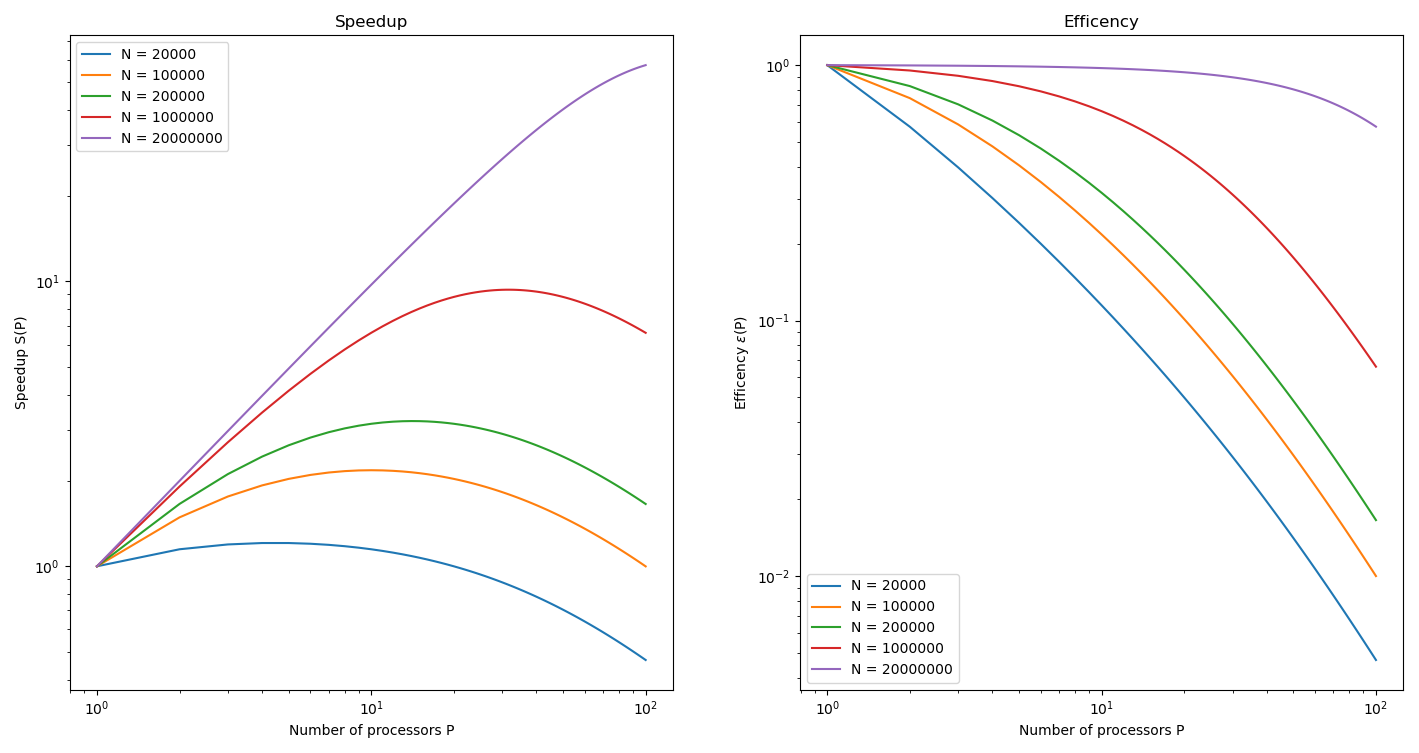
\includegraphics[scale=0.45]{Speedup_sum_naive.png}
    \caption{Left/Right speedup/efficency curves of the naive algorithm with different number of elements to be summed up}
    \label{fig:speedup_sum}
\end{figure}

As expected we see that the greater the value of N the better the algorithm scales, we riassume the number of processors that achive the best speedup for summing up N elements in table \ref{tab:speedup_sum}.\\
The table also shows the best number of processors of an enhanced version of the sum of N numbers algorithm, the idea of the algorithm is as follows:
Since the major overhead that prevents scalability is represented by the communication time, we need a better communication strategy. If the processors can communicate at the same time we can pass data or instructions around in O($\log_2P$) time. An example with 4 processors: at first processor 1 tells processor 3 to pass the instruction to processor 4 and perform the partial sum, then processor 1 tells processor 2 to perform the partial sum \textbf{while} processor 3 tells processor 4 to perform the partial sum. In this case we pass from $3\times T_{comm}$ to $2\times T_{comm}$ which isn't a big deal, but we can apply the same reasoning with an arbitrary number of processors and obtain a parallel overhead of $\mathrm{ceil}(\log_2(P))\;T_{comm}$. The same thing can be done when we send back the partial sums at the master processor.

\begin{equation}
    T_P = T_{read} + (N/P + P-1)T_{comp} + 2\;\mathrm{ceil}(\log_2(P))\;T_{comm}
\end{equation}

\begin{table}[h]
    \centering
    \begin{tabular}{ccc}
        N & best P naive & best P enhanced\\
        \hline\hline
        20000& 4 &16\\
        100000& 10 &64\\
        200000& 14 &100\\
        1000000& 32&100\\
        20000000& 100&100\\
        \hline
    \end{tabular}
    \caption{Number of processors that achive the best speedup for summing up N elements}
    \label{tab:speedup_sum}
\end{table}

\begin{figure}[h]
    \centering
    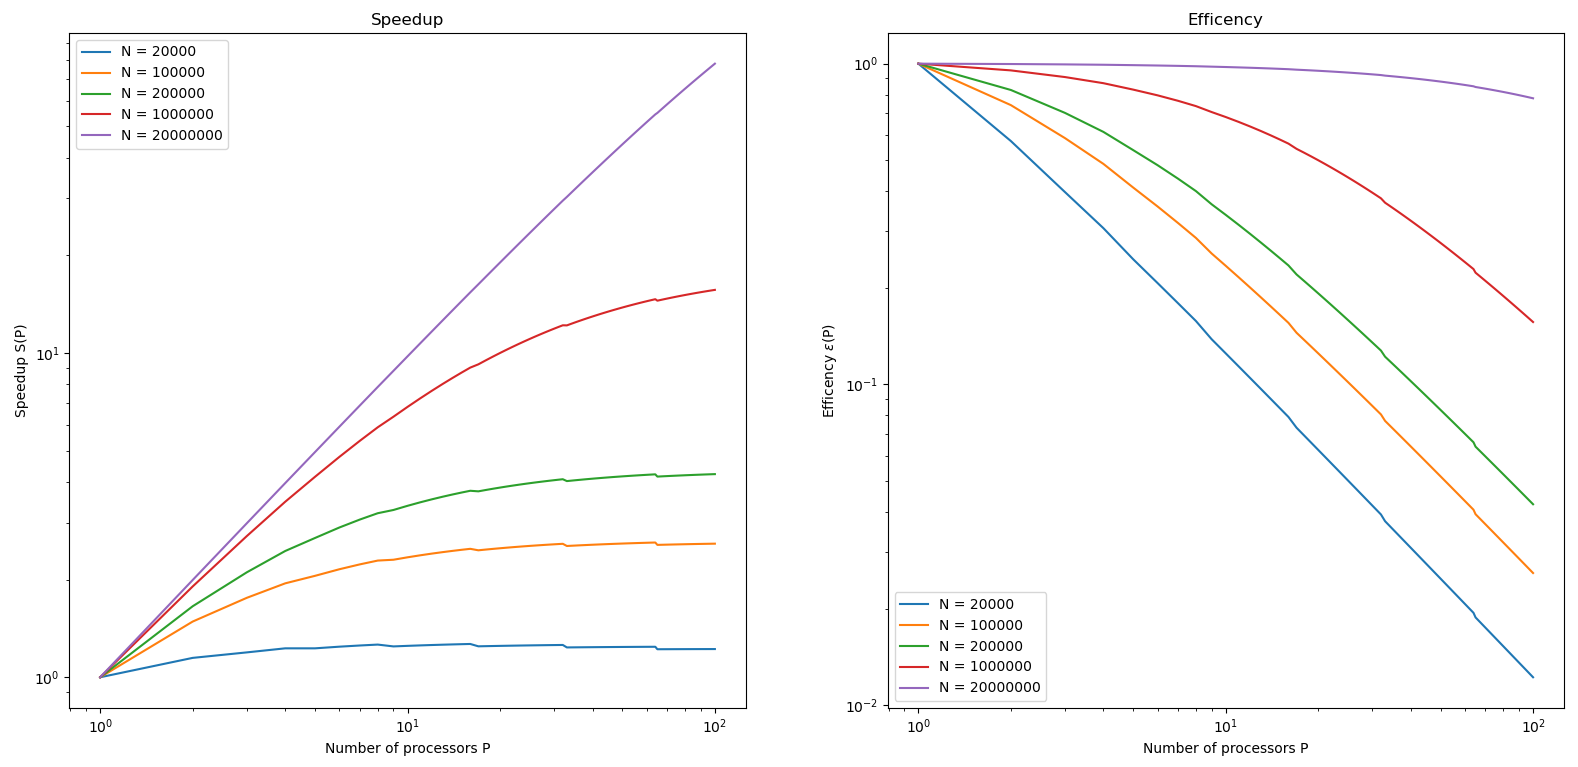
\includegraphics[scale=0.4]{Speedup_sum_enhanced.png}
    \caption{Left/Right speedup/efficency curves of the enhanced algorithm with different number of elements to be summed up}
    \label{fig:speedup_enhanced}
\end{figure}


\section{MPI program}
\subsection*{2.1 Compute strong scalability of the mpi\_pi.c program}
I ran the serial program 3 times with 100 million iterations and recorded a time $T_s=2.56\pm0.01 [s]$ using the \texttt{/usr/bin/time} command, the mpi program took instead $T_{p}=2.84\pm0.02 [s]$, we can therefore give an estimate of the parallel overhead $T_{p} - T_s = 0.28 \pm 0.03 [s]$ which is about $10\%$ of the parallel running time.

In figure \ref{fig:strong_times} I plotted the running time of the algorithm with various number of moves against the number of processors used. We see a remarkable difference, for moves=$10^8$ and $10^9$, in the time taken using the \texttt{ust/bin/time} command vs the internal time of the processors (taken by choosing the maximum among all the walltimes). This difference could be caused by mpi, in fact by looking at the \texttt{mpi\_pi.c} code we notice that after displaying the walltime the program calls \texttt{MPI\_Finalize()}, so the program doesn't end when we display the walltime. Given this we will take as the true runtime the time given by \texttt{/usr/bin/time} which has a resolution of 1 centisecond.

\begin{figure}[h]
    \centering
    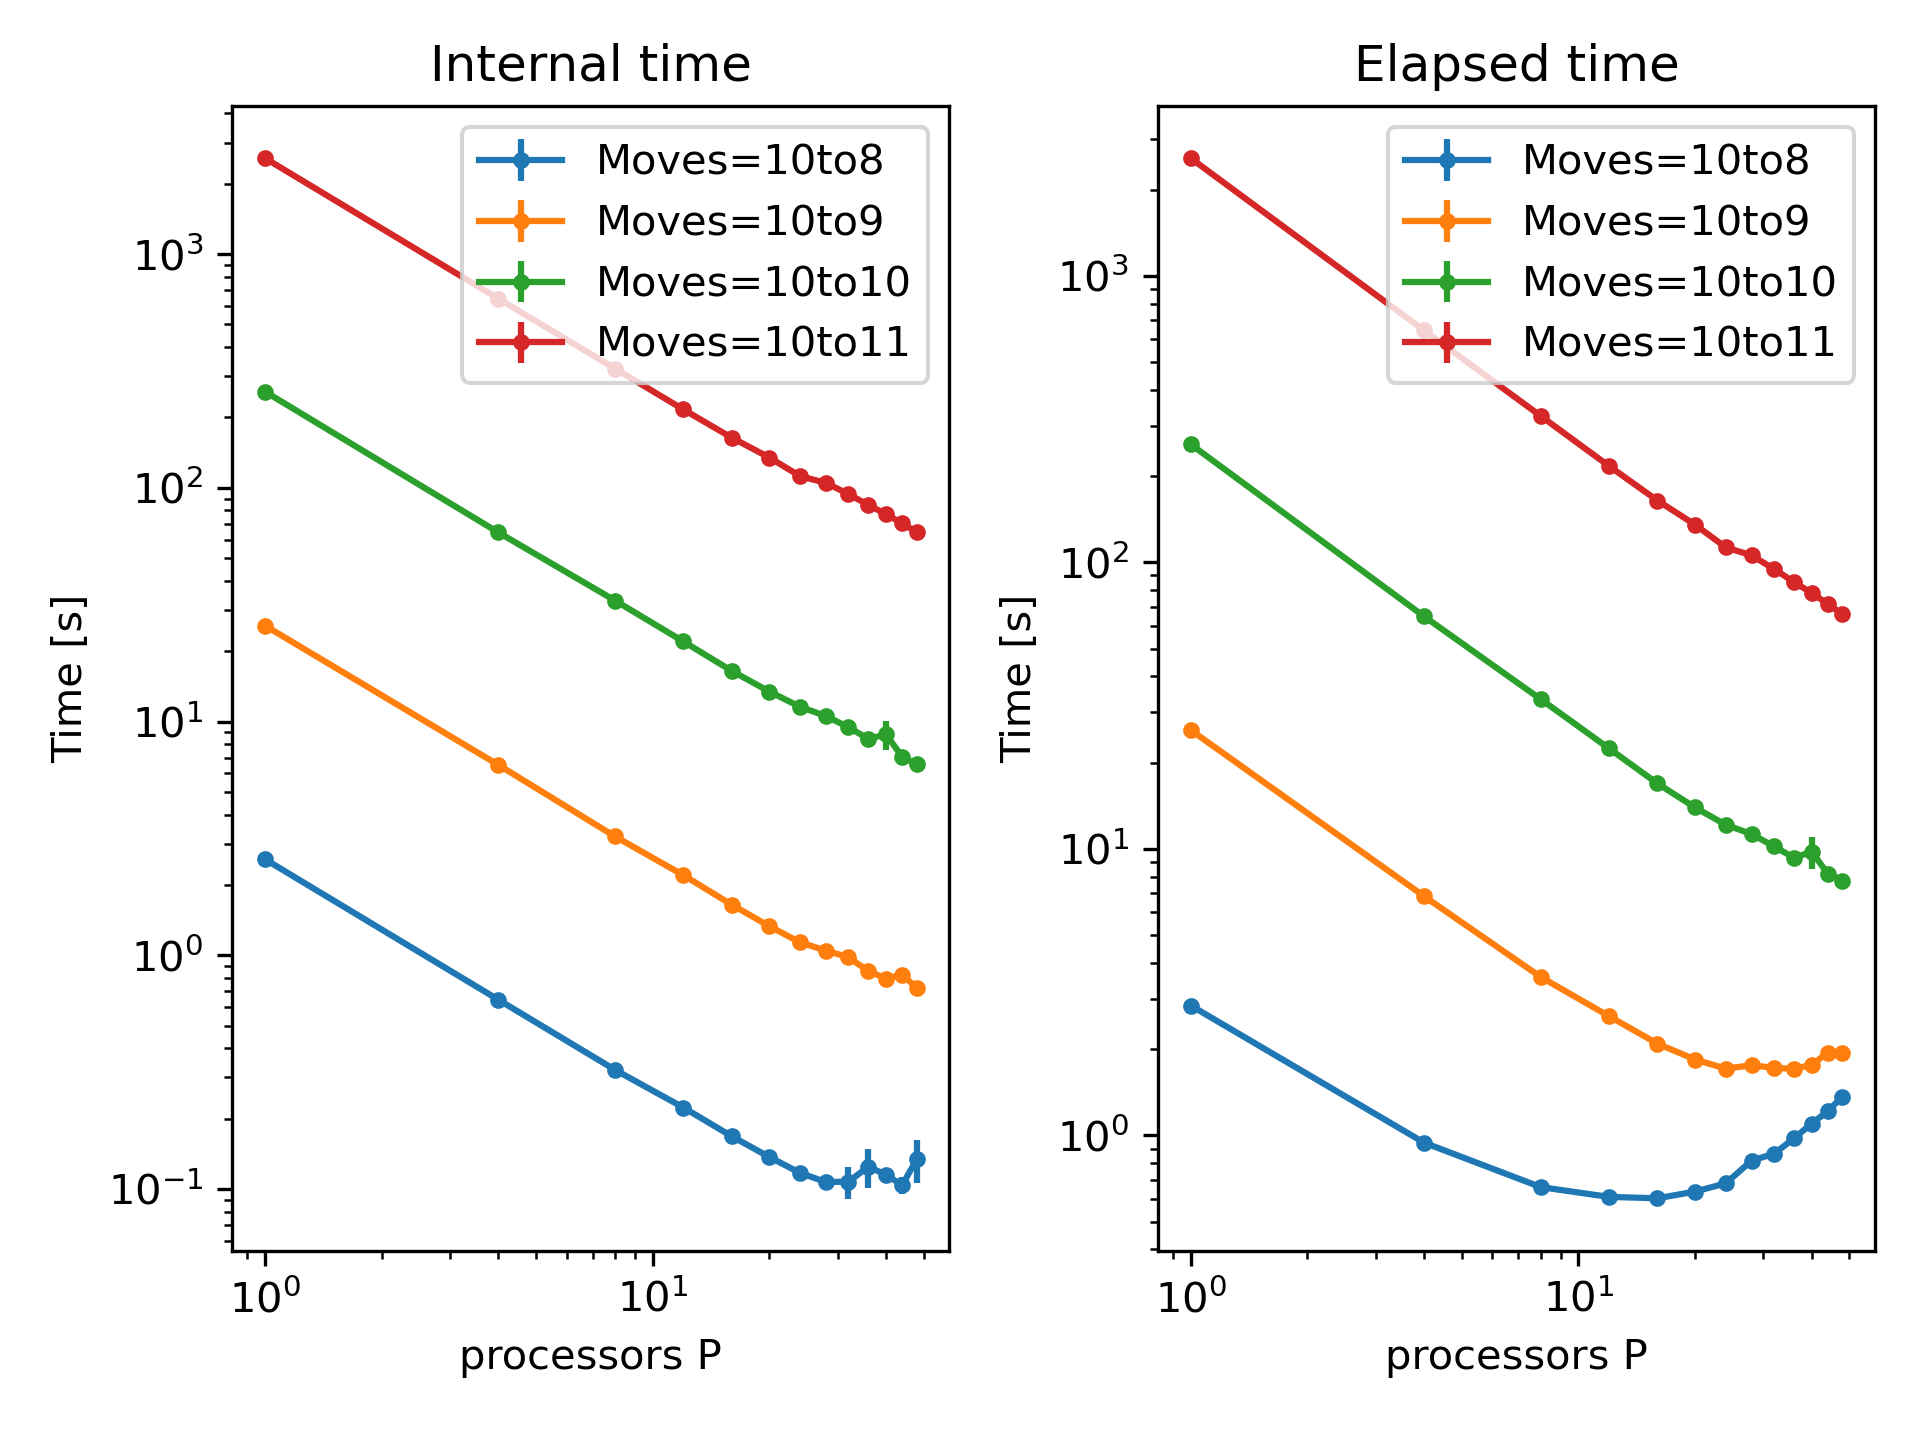
\includegraphics[scale=0.9]{strong_scaling_times.png}
    \caption{Plots of run time versus number of cores for various number of moves of the algorithm, left: plot taken using the internal time, right: plot taken using the command \texttt{/usr/bin/time}}
    \label{fig:strong_times}
\end{figure}

In figure \ref{fig:strong_speedup} I plotted the speedup curves of the algorithm with different number of moves. We notice right away the parallel overhead with $10^8$ moves discussed in section 2.1, while this isn't visible for the other number of moves. For $10^{11}$ and $10^{10}$ moves the algorithm scales almost linearly until $P\approx 24$, while this seems like a little dip in performance we have to remember that the y axis is in logaritmic scale. For moves=$10^9$ we have a plateu at about 24 processors, after which the algorithm doesn't scale anymore, finally with $10^8$ moves the program doesn't scale well, reaching a maximum speedup of 4.2 at about 16 processors. We riassume in table \ref{tab:speedup_strong} the best number processors that achieve the best speedup for the different number of moves

\begin{table}[h]
    \centering
    \begin{tabular}{ccc}
        Moves & Best P & max speedup\\
        \hline\hline
        $10^{8}$ & 16 &4.2\\
        $10^{9}$ & 36 &15.2\\
        $10^{10}$ & 48 &33.2\\
        $10^{11}$ & 48 &39.1\\
        \hline
    \end{tabular}
    \caption{Best number of processors and respective speedup for computing pi with the \texttt{mpi\_pi.c} program}
    \label{tab:speedup_strong}
\end{table}

\begin{figure}[hbt!]
    \centering
    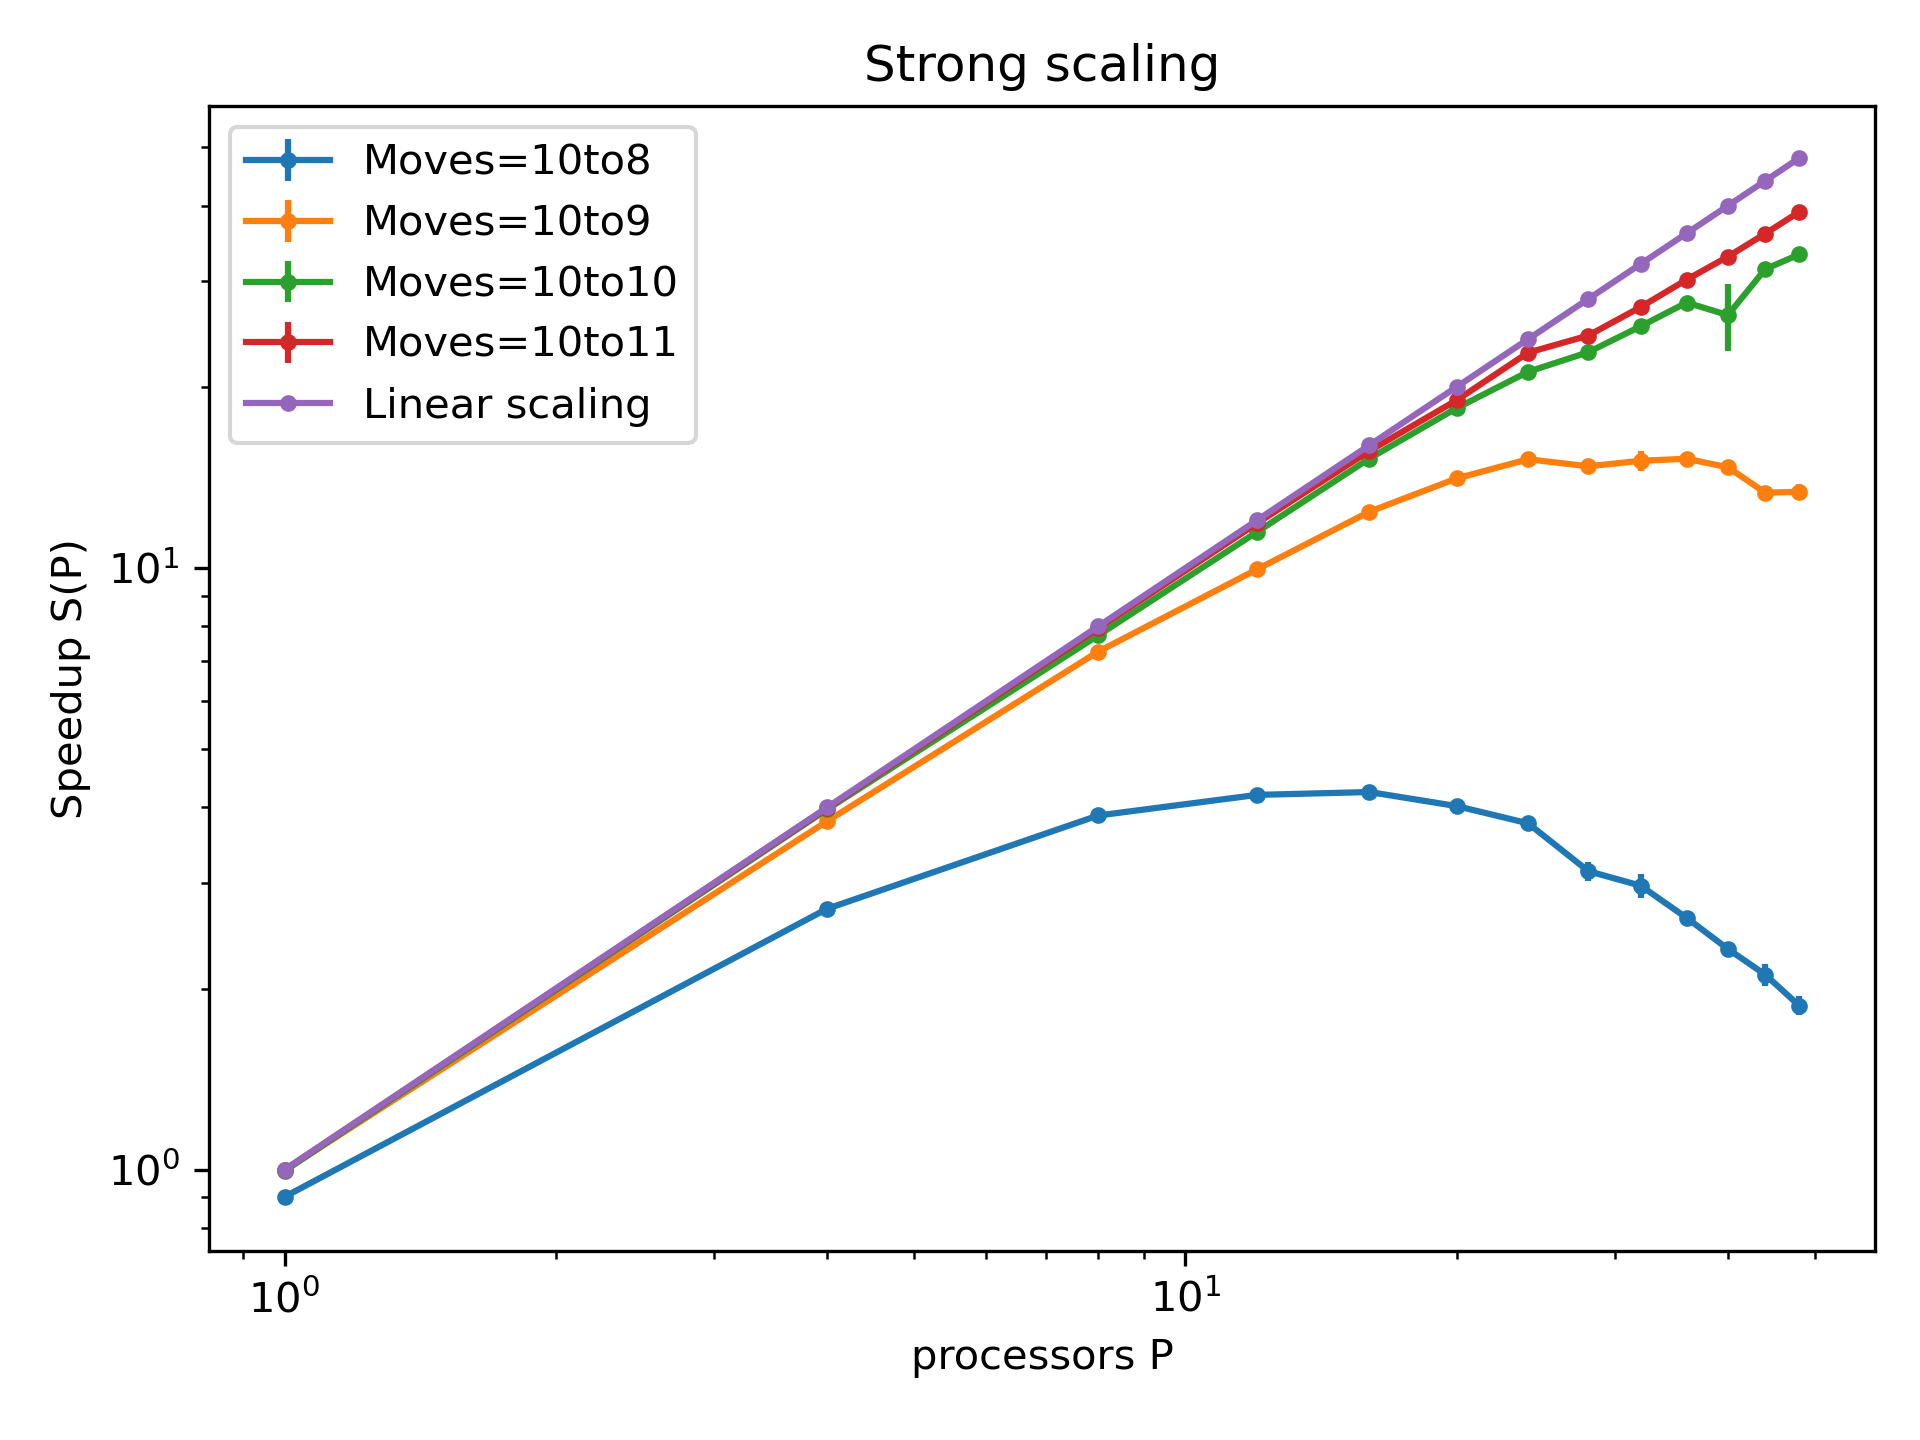
\includegraphics[scale=0.7]{strong_scaling_speedup.png}
    \caption{Plot of the speedup curves of the \texttt{mpi\_pi.c} program against number of cores for various number of moves of the algorithm}
    \label{fig:strong_speedup}
\end{figure}


\subsection*{2.2 Model for the parallel overhead}
We can adapt, with some corrections, the model of the sum of N numbers to the computation of pi. The serial time takes the form $T_S = T_{read} + N*T_{comp}$ where N are the number of moves of the algorithm, $T_{comp}$ in this case is the time to extract a random coordinate and seeing if it is inside the circle or not. The parallel time instead takes the form:
\begin{equation*}
    T_P = T_{read} + T_{mpi} + N/P \;T_{comp} + (P-1)T_{sum} + 2(P-1)T_{comm}
\end{equation*}

Where I indicated with $T_{sum}$ the time to perform a single sum and $T_{mpi}$ the overhead associated with using mpi. We then estimate the parallel overhead with the formula $T_{overhead} = T_P - T_S / P$ where the second term represents the running time of the algorithm if it scales perfectly (figure \ref{fig:parallel_overhead_time})

\begin{equation*}
    T_{overhead} = T_P - T_S / P = \frac{P-1}{P} T_{read} + T_{mpi} + (P-1)T_{sum} + 2(P-1)T_{comm}
\end{equation*}

We see that $T_{comp}$ doesn't appear in this formula since I assumed that the computation time for the serial and parallel program are the same, we can simplify further the formula by removing $T_{sum}$, since it is much smaller than $T_{comm}$, and $T_{read}$ which is much smaller than $T_{mpi}$. So the parallel overhead takes the simple form $T_{overhead} = T_{mpi} + 2(P-1)T_{comm}$, which represents a line in the plane, we perform a linear fit of the parameters to the collected data and see that for moves $10^8$ to $10^{10}$ $T_{comm}\approx 0.04/0.08 [s]$ while the value of $T_{mpi}$ doesn't count that much(the error is always very large), so we settled for the previous value of $T_{mpi}=0.28 \; [s]$. In case moves = $10^{11}$ we have $T_{comm}\approx 0.6 [s]$, an order of magnitude larger than the previous values, the model can be corrected by adding a term $aN$ with $a\approx 10^{-11}$ however I don't see the physical meaning of this term which represents a sort of penality on sustained performance.

\begin{figure}[h]
    \centering
    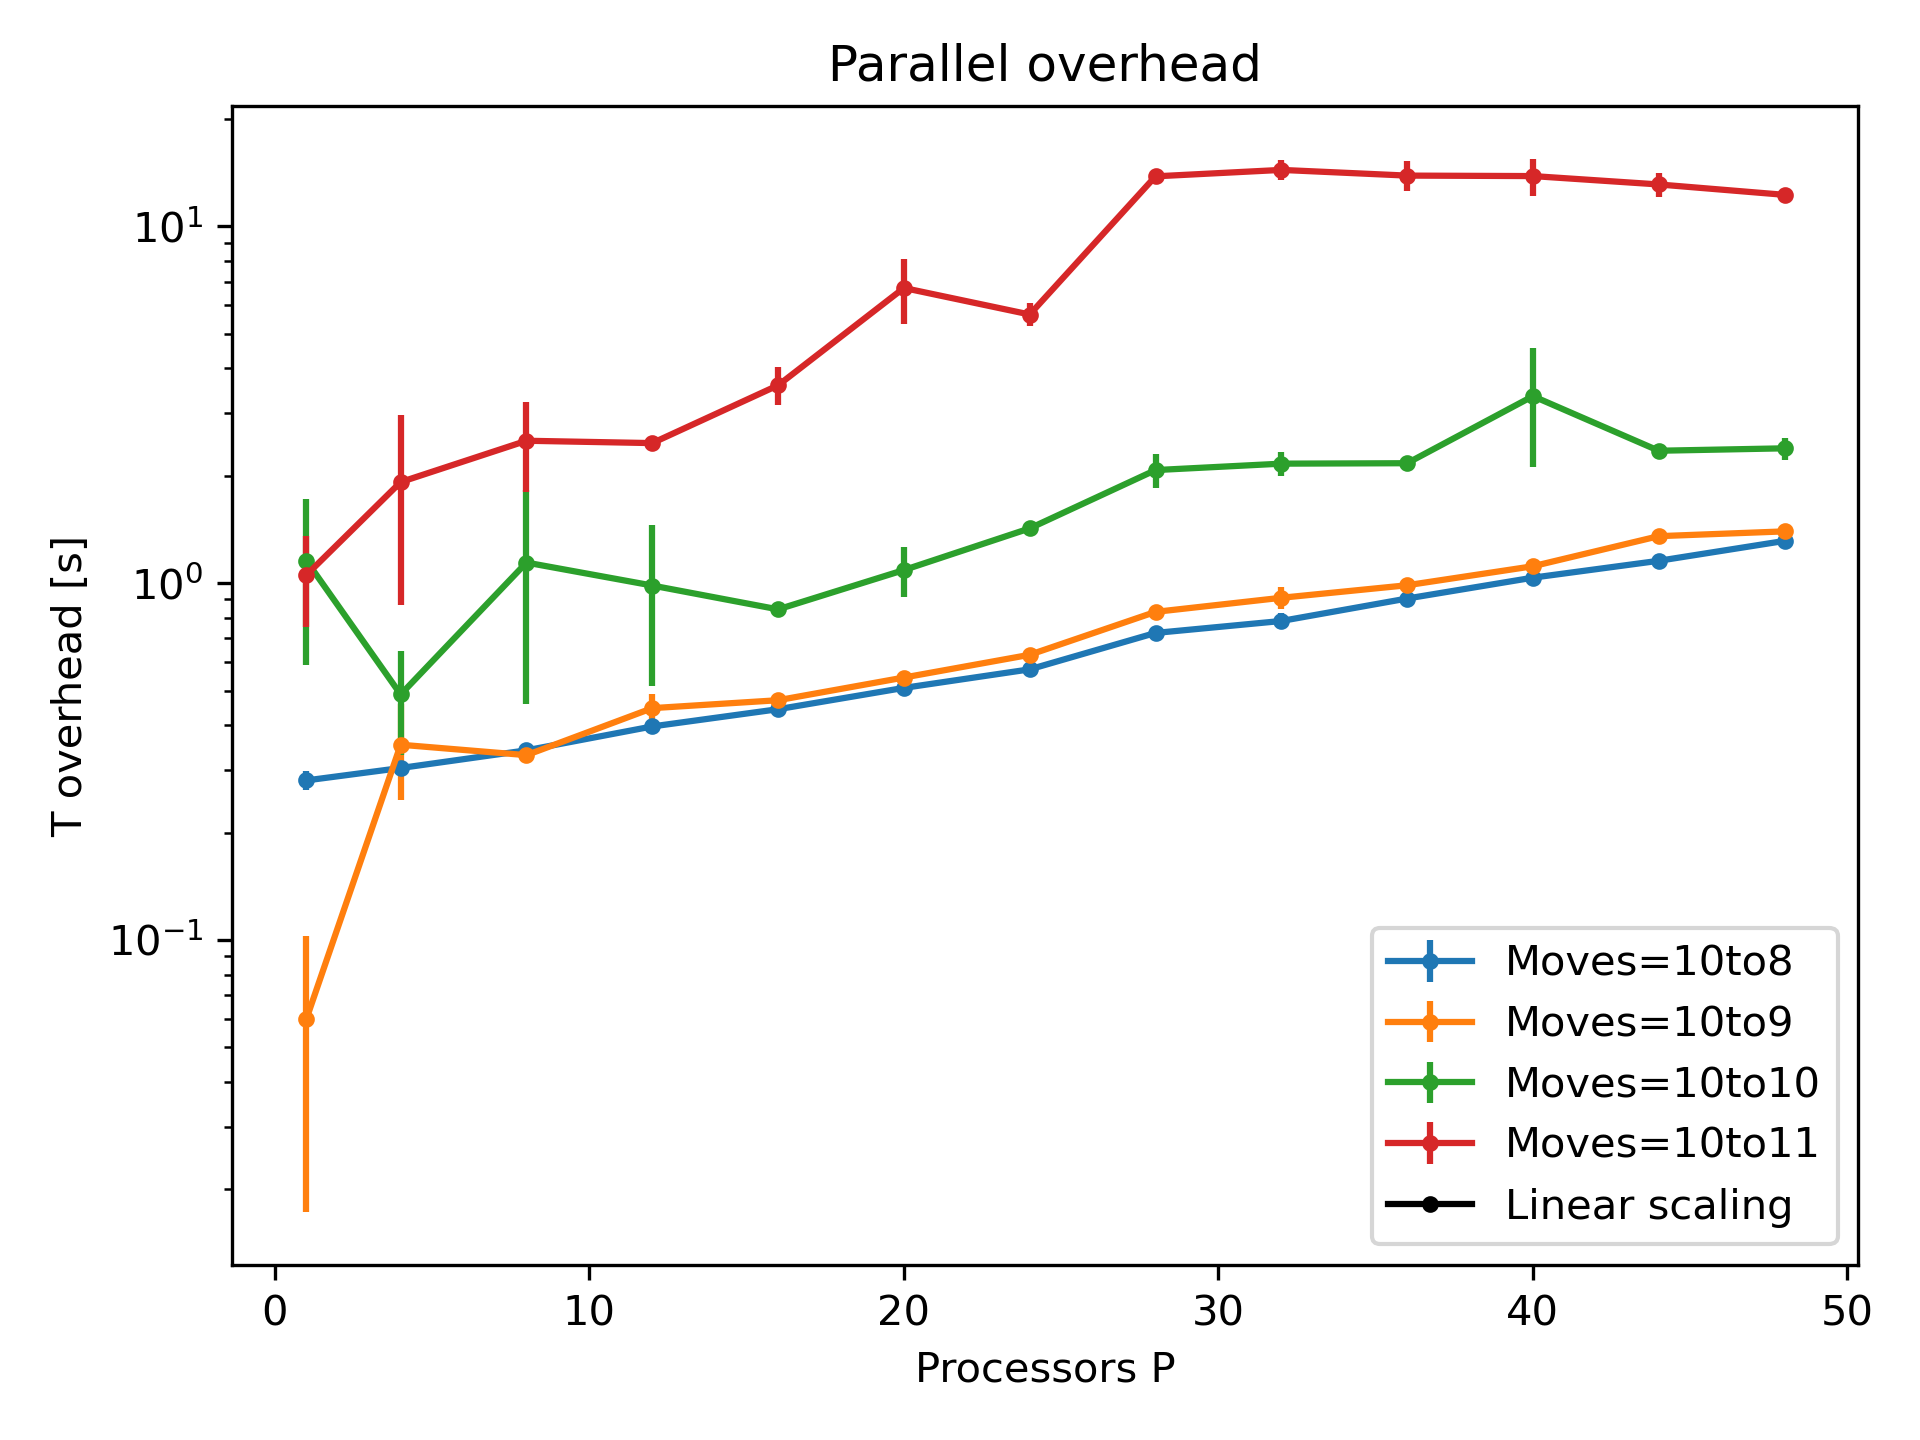
\includegraphics[scale=0.7]{parallel_overhead_time.png}
    \caption{Plots of the parallel overhead of the \texttt{mpi\_pi.c} program versus number of cores for various number of moves of the algorithm}
    \label{fig:parallel_overhead_time}
\end{figure}

\subsection*{2.3 Weak scaling}
In figure \ref{fig:weak_scaling} we see that the weak runtime increases as the processor count increases, as expected we have the worst weak scaling performance with moves=$10^8$ as can be seen from the right part of the graph, while for the other number of moves the weak efficency is roughly the same. We notice however a major drop in efficency from 24 to 28 processors, this could be due to hyperthreading because our processor has 24 physical cores, we noted the same behaviour when we discussed the strong scaling (figure \ref{fig:strong_speedup}) even though it's less noticeable

\begin{figure}[h]
    \centering
    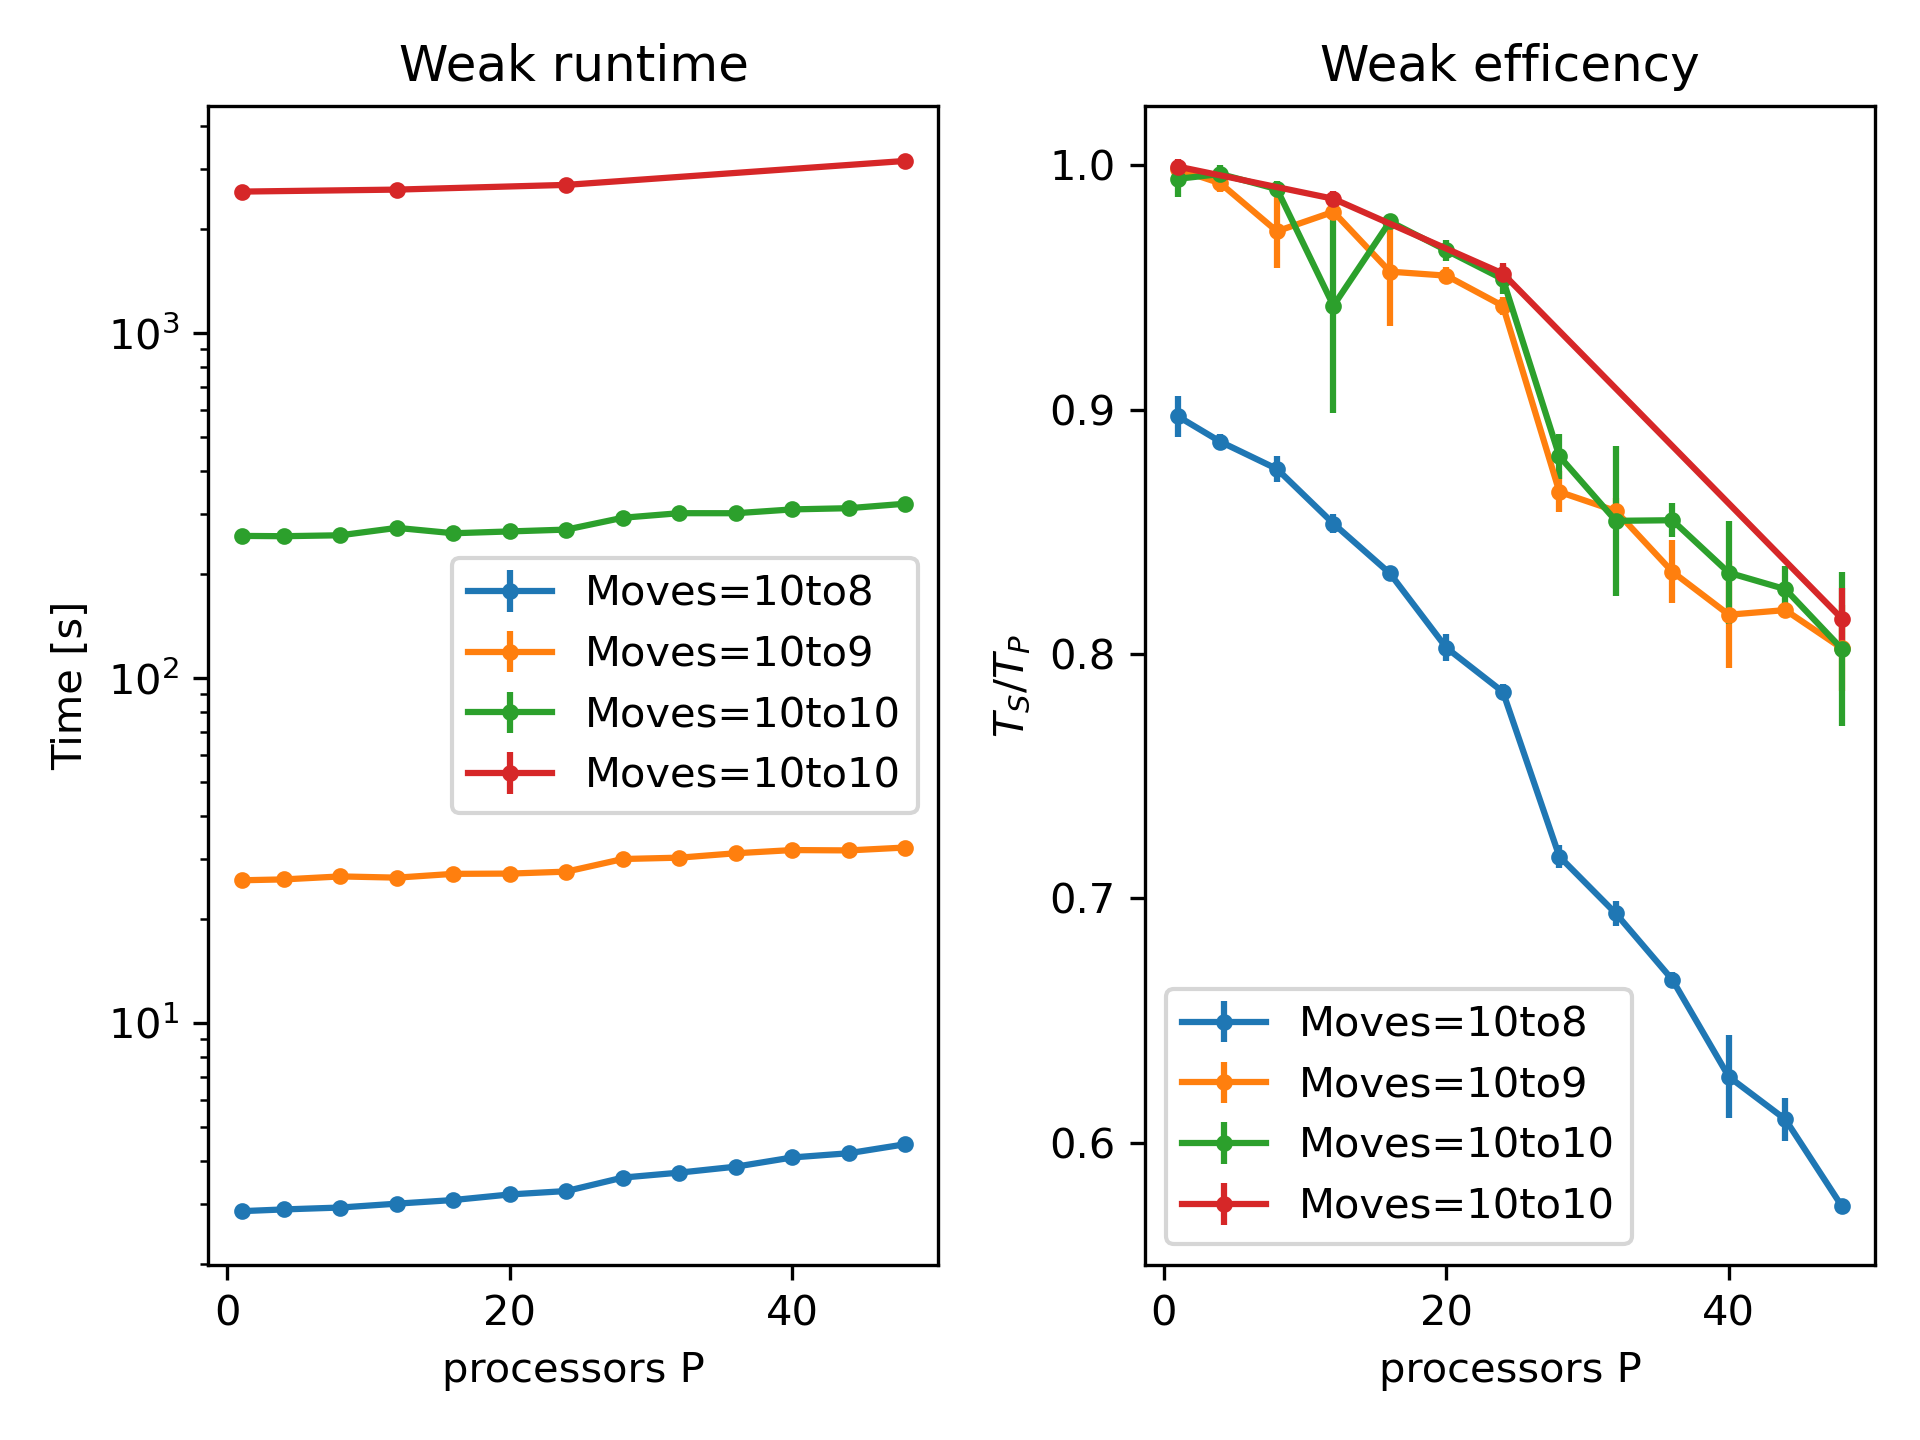
\includegraphics[scale=0.9]{weak_scaling.png}
    \caption{Right: Plot of the weak scaling time against the number of processors used. Left: Plot of the weak efficency}
    \label{fig:weak_scaling}
\end{figure}
\end{document}
